% 
% Modelo de artigo científico para a Faculdade de Tecnlogia SENAI "Mariano Ferraz"
%
% Curso de Pós-Graduação em Internet das Coisas
%
% e-mail dos integrantes do grupo:
% Rafael Gomes de Paula: rpaula@senaisp.edu.br


\documentclass[
	% -- opções da classe memoir --
	article,			% indica que é um artigo acadêmico
	12pt,				% tamanho da fonte
	oneside,			% para impressão apenas no verso. Oposto a twoside
	a4paper,			% tamanho do papel. 
	% -- opções do pacote babel --
	english,			% idioma adicional para hifenização
	brazil,				% o último idioma é o principal do documento
	sumario=tradicional
	]{abntex2}


% ---
% PACOTES
% ---

% ---
% Pacotes fundamentais 
% ---
\usepackage{lmodern}			% Usa a fonte Latin Modern
\usepackage[T1]{fontenc}		% Selecao de codigos de fonte.
\usepackage[utf8]{inputenc}		% Codificacao do documento (conversão automática dos acentos)
\usepackage{nomencl} 			% Lista de simbolos
\usepackage{color}				% Controle das cores
\usepackage{graphicx}			% Inclusão de gráficos
\usepackage{microtype} 			% Para melhorias de justificação
\usepackage{float}				% Para ajuste na posição de figuras e tabelas
\usepackage{cite}				% Para ajuste na posição de figuras e tabelas
% ---
		
% ---
% Pacotes adicionais, usados apenas no âmbito do Modelo Canônico do abnteX2
% ---
\usepackage{lipsum}				% para geração de dummy text
% ---
		
% ---
% Pacotes de citações
% ---
\usepackage[brazilian,hyperpageref]{backref}	 % Paginas com as citações na bibl
\usepackage[alf]{abntex2cite}	% Citações padrão ABNT
% ---

% ---
% Pacotes de citações
% ---
\graphicspath{ {./images/} }
% ---

% ---
% Configurações do pacote backref
% ---
% Usado sem a opção hyperpageref de backref
\renewcommand{\backrefpagesname}{Citado na(s) página(s):~}
% Texto padrão antes do número das páginas
\renewcommand{\backref}{}
% Define os textos da citação
\renewcommand*{\backrefalt}[4]{
	\ifcase #1 %
		Nenhuma citação no texto.%
	\or
		Citado na página #2.%
	\else
		Citado #1 vezes nas páginas #2.%
	\fi}%
% ---

% ---
% Informações de dados para CAPA e FOLHA DE ROSTO
% ---
\titulo{Projeto para localização de dispositivos bluetooth BLE indoor}
\autor{Josimar de Andrade Silva, \and Rafael Gomes de Paula,\and Wanderson Thiago da Silva Pagani}
\local{Brasil}
\data{24/03/2020} 
% ---

% ---
% Alterando o aspecto da cor azul
% ---
\definecolor{blue}{RGB}{41,5,195}
% ---

% ---
% Informações do PDF
% ---
\makeatletter
\hypersetup{
     	%pagebackref=true,
		pdftitle={\@title}, 
		pdfauthor={\@author},
    	pdfsubject={Projeto Localização Indoor},
	    pdfcreator={LaTeX with abnTeX2},
		pdfkeywords={abnt}{latex}{abntex}{abntex2}{artigo científico}, 
		colorlinks=true,       		% false: boxed links; true: colored links
    	linkcolor=blue,          	% color of internal links
    	citecolor=blue,        		% color of links to bibliography
    	filecolor=magenta,      		% color of file links
		urlcolor=blue,
		bookmarksdepth=4
}
\makeatother
% --- 

% ---
% Compila o índice
% ---
\makeindex
% ---

% ---
% Altera as margens padrões
% ---
\setlrmarginsandblock{2cm}{2cm}{*}
\setulmarginsandblock{2cm}{2cm}{*}
\checkandfixthelayout
% ---

% --- 
% Espaçamentos entre linhas e parágrafos 
% --- 

% O tamanho do parágrafo é dado por:
\setlength{\parindent}{.5cm}

% Controle do espaçamento entre um parágrafo e outro:
\setlength{\parskip}{0.2cm}  % tente também \onelineskip

% Espaçamento simples
\SingleSpacing
% ---

% --- 
% Cabeçalho 
% --- 
\makepagestyle{meuestilo}
  \makeoddhead{meuestilo} %%pagina ímpar ou com oneside
     {Faculdade de Tecnologia SENAI "Mariano Ferraz"}
     %{Vol. 1,  n\textsuperscript{o} 1 (2017)}
     {}
     {IoT - SSIR,  pág. \thepage}
% ---

% ---
% Margem para resumo, palavras-chave, abstract e keywords
% ---
\def\changemargin#1#2{\list{}{\rightmargin#2\leftmargin#1}\item[]}
\let\endchangemargin=\endlist 
% ----

% ---
% Início do documento
% ---
\begin{document}

% ----------------------------------------------------------
% ELEMENTOS TEXTUAIS
% ----------------------------------------------------------
\textual

% Aplica o cabeçalho em todas as páginas, excetuando-se a primeira
\pagestyle{meuestilo}

% Retira espaço extra obsoleto entre as frases.
\frenchspacing 

% Página de titulo
\maketitle

% Aplica cabeçalho na primeira página
\thispagestyle{meuestilo}
% ---

% -----------------------------------------------------------
% Resumo em português
% -----------------------------------------------------------
\begin{changemargin}{1cm}{1cm} 
 \textbf{Resumo} – A proposta do projeto é criar um sistema de localizaçao em tempo real de dispositivos bluetooth dentro de um local fechado.
 O hardware consiste na criação de um dispositivo utilizando o ESP32, capaz de localizar outros dispositivos bluetooth, como IBeacons, através da triangulação destes dispositivos que denominamos "estações de rastreamento". 
 As estações disponibilizaram as informações dos dispositivos encontrados através da internet, utilizando o protocolo MQTT e a plataforma Node-Red.
 O Software consiste em um website, construído utilizando Node.js como servidor aplicacional, capaz de se conectar ao Node-Red e fazer a interpretação dos dados.
 A plataforma é responsável por receber os dados e determinar qual é o dispositivo mais proximo dentro do raio da triangulação das estações.
 \vspace{\onelineskip}
 
 \noindent
 \textbf{Palavras-chave} – IoT; Internet das Coisas; Comunicação; Localização; Sinal; Rádio Frequência; Alarmes; Indoor 
\end{changemargin}
% ---

% -----------------------------------------------------------
% Resumo em inglês
% -----------------------------------------------------------

\begin{changemargin}{1cm}{1cm} 
\textbf{Abstract} – The project proposal is to create a real-time location system for bluetooth devices within an enclosed location. The hardware consists of creating a device using ESP32, capable of locating other bluetooth devices, such as IBeacons, through the triangulation of these devices that we call "tracking stations". The stations made available the information of the devices found through the internet, using the MQTT protocol and the Node-Red platform. The Software consists of a website, built using Node.js as an application server, capable of connecting to Node-Red and interpreting the data. The platform is responsible for receiving the data and determining which is the closest device within the radius of the triangulation of the stations
\vspace{\onelineskip}
	
\noindent
\textbf{Keywords} – IoT; Internet of Things; Comunication; Location; Signal; Radio Frequency; Alarm; Indoor 
\end{changemargin}
   
% ---

% ----------------------------------------------------------
% Introdução
% ----------------------------------------------------------
\section{Introdução}
\addcontentsline{toc}{section}{Introdução}

% ---
% Nota de rodapé na primeira página
% ---
%\let\thefootnote\relax\footnotetext{(A ser preenchido pelos editores)  Versão inicial submetida em DD de MM. de AAAA.   Versão final aceita em DD de MM. de AAAA.  Publicado em DD de MM. de AAA.  Digital Object Identifier \_\_\_\_\_\_\slash\_\_\_\_\_ }
\let\thefootnote\svthefootnote
% ---

De acordo com LIMA (2014) o primeiro sistema de identificação por radiofrequência (RFID) surgiu em 1937 com a invenção do primeiro radar, liderado pelo escocês Sir Robert Alexander Watson-Watt da United States Naval Research Laboratory.
Após a invenção do primeiro radar, a tecnologia RFID tem sido usada para diversos tipos de aplicação, como controle de segurança, monitoramento, controle de temperatura, rastreabilidade, entre outras diversas situações.
Segundo OMEGA (2020) os sensores sem fio utilizados em aplicações de localização são ferramentas de medição padrão equipadas com transmissores utilizados para converter sinais de instrumentos de controle de processo em uma transmissão de rádio. O sinal de rádio é interpretado por um receptor que converte o sinal sem fio em uma saída específica, tal como uma corrente analógica ou uma análise de dados feita por um software.  
LOUREIRO (2003) exemplifica que cada sensor possui características particulares que variam de acordo com o ambiente e objetivo do uso, sendo alguns desses sensores: com endereçamento, para mobilidade, limitação de energia e outros.
A pesquisa apresentada neste trabalho se refere aos sensores RFID, aplicados para simplificação de atividades humanas em locais indoor. Um exemplo disso são os sistemas de localização e cálculo de distância, que utilizam as propriedades da rádio frequência como um recurso para calcular a posição ou a longitude entre dois objetos.
O objetivo principal deste trabalho é demonstrar uma das técnicas baseada no sinal Bluetooth de Baixa Energia (BLE) mais utilizadas nos sensores de localização indor, a Indicação de Intensidade do Sinal de Rádio (RSSI), que utiliza, respectivamente, o tempo de chegada do sinal a uma ERB (Estação Base), o ângulo de chegada do sinal em relação às Estações de Rádio Base (ERB’s) e a intensidade do sinal, para calcular a posição de um objeto.  
Este trabalho, portanto, orientar-se-á no sentido de analisar o processo de localização de pessoas em um ambiente indor de modo a utilizar a técnica RSSI, podendo ajudar a diminuir o tempo de atuação envolvendo problemas em sistemas de missão crítica.

\section{Pesquisa Bibliográfica}
Ao desenvolver as pesquisas foi utilizado o método de revisão literária, sendo esse um método qualitativo, apoiando-se em técnicas de pesquisa de dados. Realizado pela análise de conteúdos e artigos de sites, artigos técnicos, dissertações de mestrado, pesquisas bibliográficas, manuais e normas técnicas, publicados nos períodos dos últimos 20 anos, sobre o tema em questão.
Ainda é um grande desafio para as tecnologias de localização em ambientes internos. O Sistema de Posicionamento Global (GPS), por exemplo, é uma das descobertas mais eficientes, tratando-se de tecnologias baseadas nos sensores RFID. No entanto, os metros quadrados de um ambiente indoor estão fora do alcance de seus 28 satélites (LIMA, 2001). 
Na realidade, estes ambientes não são mapeados para que um sistema de GPS possa localizá-los. Desta forma, o foco de pesquisas associadas à localização de pessoas e objetos têm se baseado na busca por tecnologias apropriadas a ambientes internos. Muitas das dificuldades estão relacionadas, já que estes locais apresentam uma estrutura que não se vê externamente, como COLEMAN e (WESTCOTT, 2009):
\begin{enumerate}
	\item Alta atenuação e difusão do sinal, devido aos inúmeros obstáculos;
	\item Mudanças temporais relacionadas à movimentação de pessoas e abertura de portas;
	\item Multipath causado pela reflexão das paredes e móveis.	
\end{enumerate}	
Por outro lado, os ambientes internos oferecem algumas facilidades, já que não sofrem interferências de fatores climáticos; podem ser facilmente mapeados e possuem melhor infraestrutura (acesso a internet e energia elétrica). Portanto, neste trabalho, o estudo da localização baseada na leitura bidirecional do RSSI será destinado a ambientes indoor.

\section{Estudo de Caso}
\subsection{Objetivo}
O objetivo do estudo de caso referente a este trabalho é demonstrar a necessidade que os data centers tem em resolver problemas de infraestrutura em um menor tempo possível e o que impacta com um problema não resolvido, influenciando na sociedade.
Para demonstrar a utilização do projeto, foi escolhido o Data Center Prodesp, considerado ambiente de missão crítica, onde em uma situação de crise na infraestrutura, o tempo de atuação dos técnicos deve ser o mais rápido possível
\subsection{Justificativa}
De acordo com ICOR (2020), existem muitos fatores de risco de paralisação nos Data Centers, como falhas naturais, humanas e de origem dos hardwares e sistemas instalados. Onde o maior percentual de causas da paralisação dos data centers são por falhas humanas. 
Devido a planta do Data Center Prodesp ser de grande escala em relação ao numero de técnicos para manter a energia elétrica constante alimentando os equipamentos de Tecnologia da Informação (TI) e equipamentos de climatização (Ar-condicionado de precisão), foi possível uma projeção para melhorar o tempo de atuação dos técnicos em um ocorrência (alarmes) com o uso de um localizador de pessoas indor por meio da tecnologia RSSI.
Considerado que a equipe de manutenção residente do Data Center Prodesp leva em média 5 minutos para localizar uma ocorrência através de um sistema supervisório Controle de Supervisão e Aquisição de Dados (SCADA), com a ajuda do localizador esse tempo pode ser menor, de acordo com a proximidade entre o técnico atuante e o equipamento em alarme. 
\subsection{Relevância para a Sociedade}
Segundo PENSO (2020), os data centers são importantes para realizar atividades simples do cotidiano, sendo desde a Internet, que você acessa para se divertir com jogos e vídeos, até os pagamentos feitos no aplicativo do seu banco, consultas de saldo e extrato, transferências ou aplicações.

\section{Definição do Projeto}
\subsection{Topologia}
A internet das coisas (IOT) proporcionou o uso do protocolo Transporte de Telemetria do Serviço de Enfileiramento de Mensagens (MQTT) para comunicação entre os hardwares de forma harmoniosa sendo possível troca de informações entre as TAG’s, ERB’s, aplicativo para celular (APP) de alarmes, software de monitoramento e servidor em nuvem. 
Segundo Zhu (2010) a origem do protocolo MQTT surgiu no laboratório Massachusetts Institute of Technology (MIT) com a pesquisa no campo de localização e identificação usando sensores sem fio, em 1999, onde deu inicio a área de estudos da Internet das Coisas.
\begin{figure}[t]
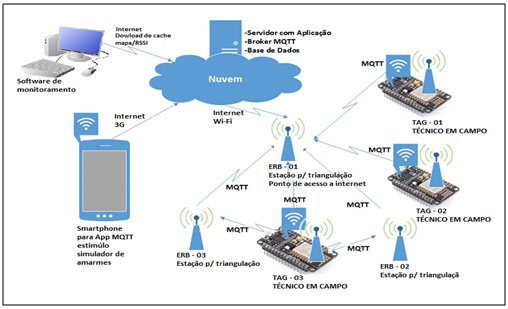
\includegraphics{topologia}
\centering
\end{figure}
Na figura 01 pode-se ver o fluxo de dados utilizando o protocolo MQTT para este trabalho.
O servidor com aplicação MQTT Node-RED da International Business Machines (IBM) recebe os estímulos de um APP que simula um possível alarme e equipamento instalado em um ambiente indor. As ERB’s verificam a intensidade do sinal RFID vindas das TAG’s IBeacons, que também são informadas sobre o alarme mais próximo.
\subsection{Hardware}
\subsection{Programa}

\section{Validação}
\subsection{Testes}
\subsection{Acertos}

\section{Resultados}
\subsection{Positivos}
\subsection{Negativos}

\section{Conclusão}
Em vista que, foi possível demonstrar como funciona e como se monitora pessoas por sistema RSSI, pode se afirmar que foi alcançado o objetivo deste trabalho.
Os objetivos foram atingidos de forma, apresentado o principal tipo e modelo de localizador indor e a sua utilização em sistema de missão crítica. Verificado o principal método de localização indor, RSSI. Através dos ensaios e testes foi possível notar a importância de um bom programa (software) a manter um nível de confiabilidade de localização, através de algoritmos podendo corrigir erros causados por ruídos.
Para trabalhos futuros sugiro que analisem outros métodos de localização com tecnologia de rádio frequência e a viabilidade econômica em manter a localização indor para grande alcance. Esse trabalho seria de grande valia também, pois demonstra a base do estudo de um sinal RFID, para avaliação da intensidade de sinal em um ambiente indor.
Pode se concluir com este trabalho que através de ensaios e testes com componentes RSSI é possível garantir a localização de pessoas, diminuindo o risco de falhas e interrupções de funcionalidade em sistemas de missão crítica, garantindo um melhor aproveitamento dos técnicos que atuam para resolver problemas em data centers.

\section*{Agradecimentos}

Dedicamos este trabalho aos amigos e professores que nos apoiaram para nossa formação acadêmica.

\bibliographystyle{plain}
\bibliography{references.bib}


\end{document}